\documentclass[10pt,a4paper]{scrartcl}
\usepackage[utf8]{inputenc}
\usepackage[english]{babel}
\usepackage{amsmath}
\usepackage{amsfonts}
\usepackage{amssymb}
\usepackage{graphicx}
\usepackage{hyperref}
\usepackage[cm]{fullpage}


  
\author{Diego Ballesteros, Tracjhe Kralev, Tribhuvanesh Orekondy}
\title{DJ Tini Data}
\subtitle{The small scale implementation of DJ Byg Data}
\date{\today}

\begin{document}
  \maketitle
  \section{Introduction}
    The general aim of this project is to develop a system able to produce
    information out of data extracted from songs. This is the general
    aim of the research field known as Music Information Retrieval (MIR),
    this field has been active for quite some time \cite{nameThatTune:1993}
    and its applications can be seen in several commercial products such as
    Pandora or Spotify \cite{recommendation:2010}.

    A great portion of the activity in MIR deals with song meta-data and audio
    features \cite{McFee:2012:MSD:2187980.2188222}. However, in this project we
    focus on lyrics as the main source of data.
    The main task that we pursue is to answer the following question:
    
    "Is it possible to determine the genre of a song based solely on its
    lyrics?"
     
    In order to accomplish this, we first explored how to extract genre
    information from the songs' lyrics and then evaluated the quality of the
    judgments. Lastly we made the developed methods available as a web
    application where arbitrary lyrics can be input in order to obtain
    a genre prediction.
    
    The report is organized as follows, first we present the input datasets used
    for the task and their respective pre-processing and manipulation. We then
    proceed to briefly explain the computing and analysis techniques chosen for
    the task. In the third section we present details of the implementation of
    these techniques. Finally the obtained results and the performance of the
    algorithms is discussed.
  \section{Data}
  
    \subsection{Description} \label{sec:data:subsec:description}
    In order to carry out the previously stated task, we selected the Million
    Songs Dataset (MSD) \cite{Bertin-Mahieux2011}.
    This dataset is a free collection of audio features and metadata for a million
    of tracks, it was collected by the LabROSA at Columbia University using
    the EchoNest API
    \footnote{\url{http://the.echonest.com/}}.
    
    However, the main dataset contains only song metadata
    (e.g. artist and album) and audio features which are not of interest
    for this project. Fortunately, the dataset is accompanied by four companion
    datasets:
    
    \begin{description}
      \item[SecondHandSongs] List of cover songs within the MSD.
      \item[Taste profile] User data from EchoNest for a subset of the MSD.
      \item[musiXmatch] Lyrics for the songs in the MSD
                        \footnote{Lyrics are available only in bag of word
                                  representation due to copyright.}.
      \item[Last.fm] Tags and similarity information for songs in the MSD.
    \end{description}
    
    Of interest for the current task are the last two datasets. The musiXmatch
    dataset provides the lyrics needed for the analysis and the Last.fm tags can
    be used to identify the genre of the songs.
    
    Summarizing, the data to be used is:
    
    \begin{itemize}
      \item The main MSD, only the IDs are used. There are 1M in the
            dataset and its uncompressed size is of about 280GB.
      \item The musiXmatch dataset has lyrics for almost 240k songs from the
            MSD. The reasons for the reduced size are: copyright, duplicates and
            instrumental tracks.
      \item The Last.fm dataset includes 94\% of the songs in the MSD, and in
            total around 500k have at least one tag.
    \end{itemize}

    \subsection{Downscaling}
    For this first milestone, we were tasked with selecting subset that can
    run in a single machine. In this case, the selection was straightforward
    since there is a 10k randomly sampled subset available in the MSD website.
    We considered this an appropriate size for the initial task.
    
    For the Last.fm dataset it was also possible to get the matching 10k
    subset but for the musiXmatch we needed to download the whole dataset
    with the 240k songs' lyrics.
    
    The sizes and formats of these subsets are listed in table
    \ref{tab:size_subset}.

    \begin{table}
      \center
      \caption{Sizes and formats for the data subsets}
      \begin{tabular}{|c|c|c|}
      \hline
      Dataset & Format & Size (GB) \\
      \hline
      MSD & Text files & 2.6 \\
      Last.fm & SQLite & 0.5 \\
      musiXmatch (Full) & SQLite & 2.3 \\
      \hline
      \end{tabular}
      \label{tab:size_subset}
    \end{table}

    \subsection{Preprocessing}
      In order to have a consistent access to all the information per track,
      we processed the input text files and SQLite databases and merged them
      into a single text file where each line is a JSON object with the
      track ID, its associated genres and the word frequencies for its
      lyrics.
      
      Here it was necessary to filter out the tracks without any genre information
      or less than 10 words in its lyrics, after this filtering the subset
      shrank to 1.4k songs and in its JSON representation it had a size of 1.1MB.
      
      \subsubsection{Discovering genres in tags}    
        As mentioned in \ref{sec:data:subsec:description}, the Last.fm provides us
        with human-made tags, these tags however contain all sorts of information
        and are not focused on genres only. In order, to use these
        as ground truth for the experiments we cleaned the tags by comparing
        them against a comprehensive online list of genres
        \footnote{\url{http://www.musicgenreslist.com/}}.
        In order to capture possible misspellings we considered a tag equal to
        a genre in the list if their Damerau-Levenshtein distance
        does not exceed 1.
      
  \section{Design}  
    \subsection{Algorithms}
      For this milestone we explore two approaches, namely clustering and
      locality sensitive hashing.
      \subsection{Clustering}
        In order to classify a set of songs as belonging to one particular
        genre, we chose the unsupervised learning technique of clustering
        as one possible solution.
        Our goal is to create a set of clusters covering the set of all songs
        with lyrics and then using the clean genre tags determine the genres
        that are the majority in each cluster.   
        The intuition here is that if a genre is present in a 50\% majority
        of the songs in cluster, then the songs can be classified as belonging
        to that genre.
      \subsection{Locality Sensitive Hashing (LSH)}
      Locality Sensitive Hashing is a popular technique used to solve the Nearest Neighbour problem in extremely high dimensional spaces.
      Given that we too deal with finding clusters, or similar neighbours of songs in a 5000-dimensional space, we consider applying LSH to solve our problem.
      
      The intuition behind LSH is that similar items are hashed to the same bucket.
      Hence by looking at the buckets, we can detect collisions, or in our case, a cluster of songs that share similar vocabulary.
      
      In contrast to k-means clustering, LSH can be implemented by making a single pass over the data.
      This in turn will help us later analyse whether k-means is worth the computational overhead.
    \subsection{Evaluation \& Metrics}
      Clustering validation techniques usually rely on specific problem
      knowledge as it is sometimes the case that the cluster metrics
      that the algorithms minimize do not reflect on the quality of the
      clusters when their information is processed by humans
      \cite{halkidi2001clustering}. 
      
      In this particular task we made use of the cleaned genre tags to define a
      metric that intuitively rates the quality of the cluster for genre       
      prediction. This metric is defined as the ratio between the number of
      clusters with at least genre that is present in more than 50\% of the
      tracks in the cluster, and the total number of clusters. This
      suggests the number of good clusters for identifying genres of
      songs, and the goal is to have a high number of good clusters.
      This metric is presented in equation \ref{eq:majority_metric}.
      
      \begin{equation}
        \label{eq:majority_metric}
        Q = \frac{\#good\ clusters}{\#clusters}
      \end{equation}
      
  \section{Implementation}
    This section describes the details of the implementation of the algorithms
    outlined above. The code for this implementation was written in its majority
    in python, along with some parts written in Javascript, HTML and CSS,
    namely the web frontend.

    \subsection{Clustering in a single machine}
      In order to perform clustering in the input data, first it is necessary to
      define a representation for the data and a distance metric in this
      representation. Since we are dealing with lyrics, which are text documents
      representing the songs, we decided that using a TF-IDF vector
      representation is a sensible choice.
      
      The term frequency (TF) calculation and smoothed inverse document frequency
      (IDF) are presented in equations \ref{eq:tf} and \ref{eq:idf},
      respectively. Where $d$ represents a document and $t$ a term.
      
      \begin{equation}
        \label{eq:tf}
        tf(d, t) = \sqrt{count(d, t)}
      \end{equation}
     
      \begin{equation}
        \label{eq:idf}
        idf(t) = 1 + \log{\frac{\#tracks}{\#tracks\ containing\ t + 1}}
      \end{equation}
      
      Finally, the TF-IDF value is simply the product of the TF and IDF.
      
      After the vectors were calculated and normalized, they were stored in
      a text file for further processing. The next step in the implementation
      is the clustering itself.
      
      For the clustering we chose K-means since it is a well known algorithm
      to approximate the optimal solution to the clustering problem
      of minimizing the sum of the distances from each point to the closest
      cluster center. We used scikit-learn
      \footnote{\url{http://scikit-learn.org/}} implementation of K-means and
      tuned the parameters to obtain the best results.

      \subsubsection{Clustering in Hadoop}
        This current approach runs well in a single machine with the current
        subset of the data, as it will described in the results section,
        however as we look forward to scale up the data size, it is necessary
        to consider changes in the algorithm.
        
        One possible variation of the clustering algorithm that has a
        straightforward implementation in a distributed computing environment,
        such as Hadoop's MapReduce, is the use of coresets to do a weighted
        sampling of the data before running a clustering algorithm on these
        samples \cite{feldman2011scalable}.
    \subsection{LSH in a single machine}
    \begin{figure}[htbp]
 	\centering
	 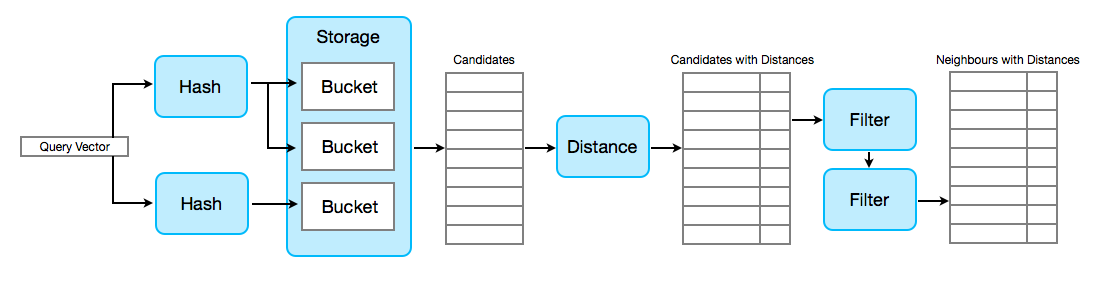
\includegraphics[scale=0.4]{img/lsh_pipeline.png}
 	\caption{NearPy's LSH pipeline (source: www.nearpy.io)}
	 \label{figure:lsh_pipeline}
      \end{figure}
    We use the library NearPy to perform Locality Sensitive Hashing on our dataset.
    This option proved quite convenient, since the project is well-documented, active and provides an already optimised single-node implementation.
    
    NearPy works as shown in Figure \ref{figure:ssh_pipeline}. 
    Given an input vector, hashes are used to generate bucket keys to which the input hashes to.
    At query time, the vector is paired up with all the candidate vectors that's contained in the respective buckets.
    After the candidates have been collected, a distance metric (Euclidean in our case) is used to identify the nearest neighbours.
    
    In our implementation of LSH, we make two passes over the dataset.
    First pass to hash the vectors to their respective buckets.
    Followed by a second pass, where each track acts as a query and identifies the nearest neighbours.
    The query vector and the neighbours are then treated as a single cluster.
      \subsubsection{LSH on Spark}
      Apache Spark's MLLib does not provide LSH out-of-the-box.
      This is complicated by the fact that NearPy's implementation does not scale to multiple machines, although the algorithm is inherently scalable.
      Hence, we intend to develop our own simplified version of LSH using Python for the next milestone.
  \section{Results}
    \subsection{Quality of results}
      \subsubsection{K-Means}
      \subsubsection{LSH}
      \begin{figure}[htbp]
 	\centering
	 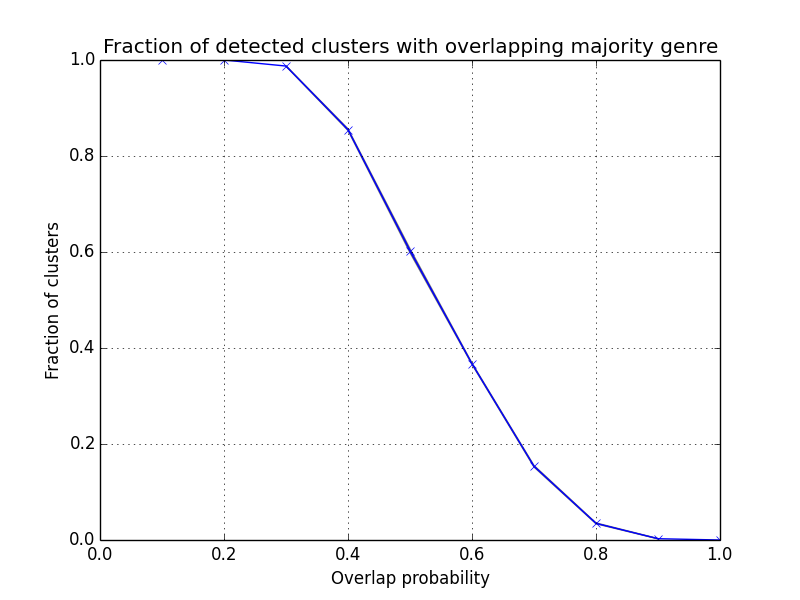
\includegraphics[scale=0.5]{img/lsh_maj_prob.png}
 	\caption{Majority genre cluster quality vs. fraction of cluster adhering to the majority genre. The graph was obtained over a series of 10 experiments, with varying hash functions.}
	 \label{figure:lsh_res}
      \end{figure}
	 
      Figure \ref{figure:lsh_res} summarizes the accuracy of LSH to detect genres based on lyrics.
      The y-axis denotes our quality metric majority genre cluster quality, which expressed what fraction of the cluster adhere to the majority genre exhibited by that cluster.
      In other words, if the overlap probability is 0.5, it implies that at least half of the tracks have a genre in common.
  \bibliographystyle{acm}
  \bibliography{report_1}
\end{document}